\section{Comparison of models and training schemes}
\label{sec:models}

Although the task of our network is to classify individual data points, we can make a small adjustment to the RNN so we can compare its performance with the more commonly used CNN in the task for which the CNN is generally applied. The CNN proposed by \cite{pearson2018searching} was evaluated on its accuracy of classifying entire light curve segments as signal or non-signal. To obtain a single classification of the RNN for an input light curve segment, we have two options. Either we take the maximum value of the corresponding PTS as prediction and make no changes to the network or training, or we train the network to output its classification over the entire segment only at the last time step. The latter approach, we refer to as ``naive'' because we only provide a sparse learning signal to the network, even though we have the option to provide a learning signal at every time step. 

\begin{table}[]
\label{tab:identification}
\centering
\begin{tabular}{@{}lccc@{}}
\toprule
Model &
  \begin{tabular}[c]{@{}c@{}}Segment accuracy\\ ($N=500$)\end{tabular} &
  \begin{tabular}[c]{@{}c@{}}Segment accuracy\\ ($N=1500$)\end{tabular} &
  \begin{tabular}[c]{@{}c@{}}Data point accuracy\\ ($N=1500$)\end{tabular} \\ \midrule
MLP           & 0.6846 $\pm$ 0.0007 & 0.60 $\pm$ 0.01   &                     \\
CNN           & 0.692 $\pm$ 0.008   & 0.61 $\pm$ 0.03   &                     \\
GRU-1 (Naive) & 0.64 $\pm$ 0.10     & 0.507 $\pm$ 0.006 &                     \\
GRU-1         & 0.68 $\pm$ 0.02     & 0.64 $\pm$ 0.01   & 0.935 $\pm$ 0.001   \\
\textbf{bi-GRU-1}      & \textbf{0.719} $\pm$ 0.003   & \textbf{0.681} $\pm$ 0.004 & \textbf{0.9399} $\pm$ 0.0003 \\
bi-GRU-2      & 0.712 $\pm$ 0.005   & 0.66 $\pm$ 0.03   & 0.938 $\pm$ 0.003   \\
bi-LSTM-1     & 0.708 $\pm$ 0.005   & 0.59 $\pm$ 0.04   & 0.931 $\pm$ 0.003   \\ \bottomrule
\end{tabular}
\caption{The comparison of different models applied to LCSim-500 and LCSim-1500, which consist of light curve segments spanning respectively 16.7 hours and 50 hours in time. The center columns show the test accuracy of classifying entire segments as signal or non-signal, similar to \cite{pearson2018searching}. The last column shows the accuracy of classifying individual data points as signal or non-signal, which is high by default because of the large data imbalance. The classification threshold in each case was set at 0.5, meaning that a segment or data point is classified as signal if the network output is larger than 0.5. Each RNN, except the naive RNN, uses the maximum of the PTS for the classification of the entire light curve segment. The values given are the means and standard deviations over three independent runs of each model.}
\end{table}

Table \ref{tab:identification} shows that the RNN (bi-GRU-1, i.e. single-layer bidirectional GRU) outperforms the CNN that was used in the comparison. It must be noted however, that the performance of the CNN depends on many hyperparameters (e.g. number of layers and channels, kernel sizes, pooling sizes, strides), and the one used here differs from the one used by \cite{pearson2018searching} because it led to better results in our case. Each network architecture was obtained by changing the hyperparameters in small steps until no large improvements were observed on the validation accuracy. To have a more consistent baseline than CNN, we also include an MLP in the comparison, similar to \cite{pearson2018searching}, which depends on fewer hyperparameters. Other models, such as two-layer GRU or LSTM are also included in the comparison as a means to motivate our choice for the bi-GRU-1. Each architecture used ReLU activation functions and a learning rate between 0.005 and 0.008. The MLP had three layers with 128, 64 and 64 nodes respectively and a weight decay of $\num{5e-3}$; the CNN had three convolutional layers with 4, 12 and 1 channels and corresponding kernel sizes of 7, 7 and 3 with strides of 1. Batch normalization and max pooling was applied between layers. The last layer of the CNN is an FC-layer with 48 nodes. Both the CNN and the naive RNN had a weight decay of $\num{1e-4}$. For all RNN variants, we used 64 nodes in the recurrent cell, which is followed by two FC-layers of both 64 nodes. 

The results also show that the preferred model (i.e. bi-GRU-1) copes well with longer input sequences, whereas the CNN is affected more strongly by the increase of data points. This is reassuring, as our network should be able to cope with long input sequences which contain more distracting background patterns than the smaller inputs the CNN is generally applied to. Moreover, the results suggest that bidirectionality is important and that simple architectures, e.g. a single recurrent layer instead of multiple layers, are preferred over more complex ones.

To further explore the potential of the RNN in the task of transit detection at the level of individual data points, we evaluate different weighting schemes during training to deal with the imbalances in the data for this task. First, we vary the positive weight $p_t$ in Figure \ref{fig:lcsim_weight_p}. The results suggest that setting a positive weight $p_t > 1$, is beneficial in terms of the tradeoff that can be made between precision and recall. The weight $p_t=12.6$ would effectively fully balance the data, because there are about 12.6 times more non-signal data points in LCSim-1500 than there are signal data points. However, as is clear from the figure, a weight this high would also require us to set a high classification threshold to obtain reasonable precision (e.g. $>$0.5). Therefore, we prefer a lower weight, e.g. $p_t = 3$, because it still increases the AP compared to $p_t = 1$, and it allows for setting a more intuitive classification threshold compared to $p_t = 12.6$.
\begin{figure}
    \centering
    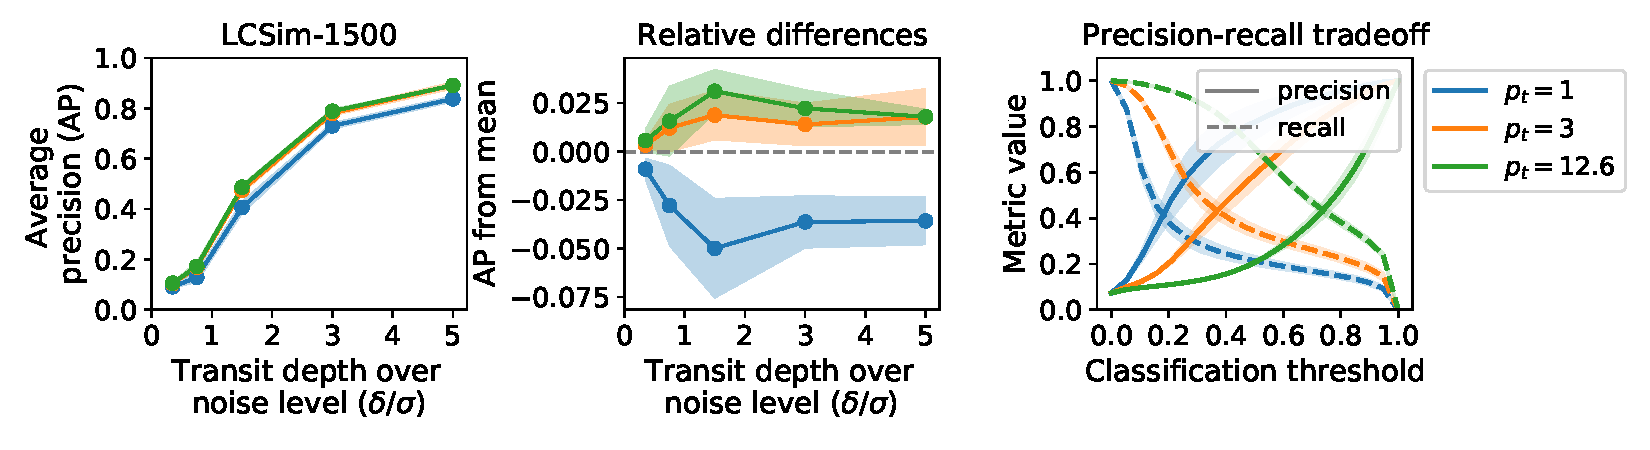
\includegraphics[width=0.95\linewidth]{Experiments/Figures/Models/lcsim1500_AP_weighting-p.pdf}
    \caption{The effect of different positive weights on the AP evaluated on the test split of LCSim-1500, and the corresponding shifts in precision and recall versus the classification threshold. To clarify, a threshold of 0.25 would mean that data points are classified as signal if the corresponding RNN outputs are above 0.25. Filled regions indicate the standard deviation over the results of three independent runs. Values between brackets show the overall AP per method.}
    \label{fig:lcsim_weight_p}
\end{figure}

Lastly, we evaluate the use of the transit-specific weighting parameter $w_{ij}$. In the simple case we have $w_{ij} = 1$, meaning that all signal data points are weighted the same, regardless of their corresponding transit depths. If the data set contains more shallow than deep transit signals, which is true in our case, then using the same weight for all transits might cause the network to become biased toward only detecting shallow signals, even though we should expect the network to perform well also in the simpler case of deep transit signals. Therefore, we evaluate setting $w_{ij} = \delta_{ij}/\sigma_i$, which sets a weight on transit samples that grows linearly with the corresponding transit depth relative to the white noise. Additionally, we set $w_{ij} = \sqrt{\delta_{ij}/\sigma_i}$, which has a similar, but less strong effect. Figure \ref{fig:lcsim_weight_w} shows that $w_{ij}$ can indeed be used to tune the focus of the network towards specific transit samples. In our case, $w_{ij} = \sqrt{\delta_{ij}/\sigma_i}$ provides a good balance in classifying transit signals of varying depths. Similar results are observed for the different weighting schemes applied to Lilith data in Figure \ref{fig:lilith_weighting}.

\begin{figure}
    \centering
    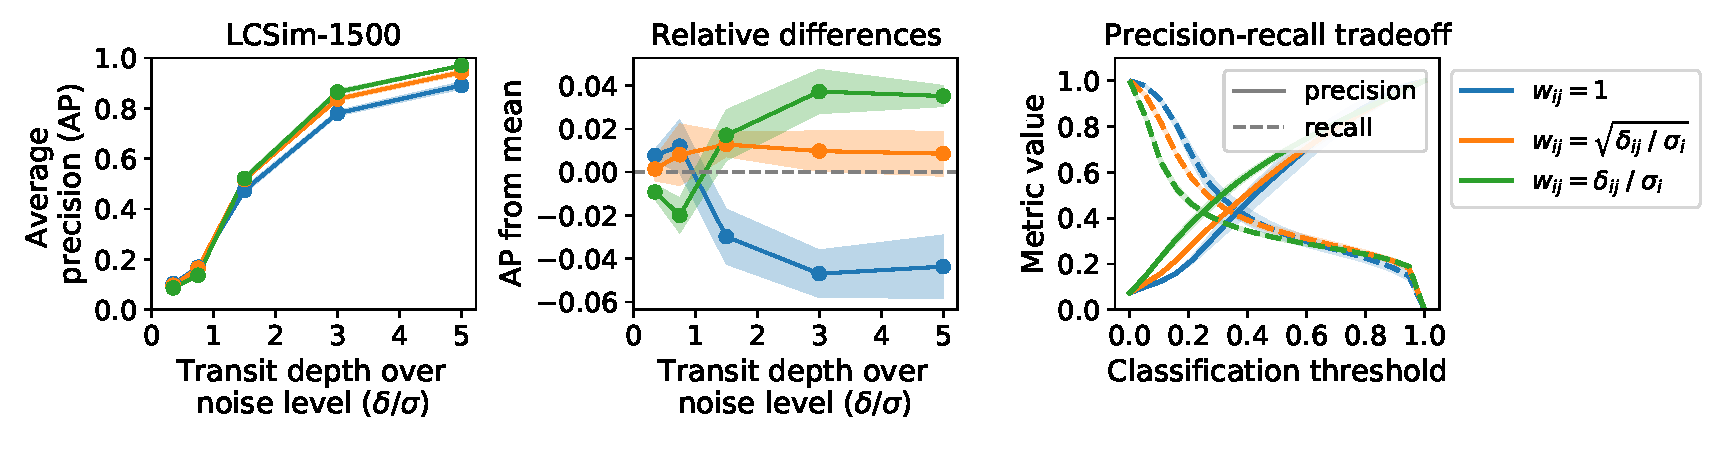
\includegraphics[width=0.95\linewidth]{Experiments/Figures/Models/lcsim1500_AP_weighting-w.pdf}
    \caption{The effect of different transit-specific weights on the AP evaluated on the test split of LCSim-1500. No large shifts in precision or recall over the classification threshold are observed. }
    \label{fig:lcsim_weight_w}
\end{figure}

\begin{figure}
    \centering
    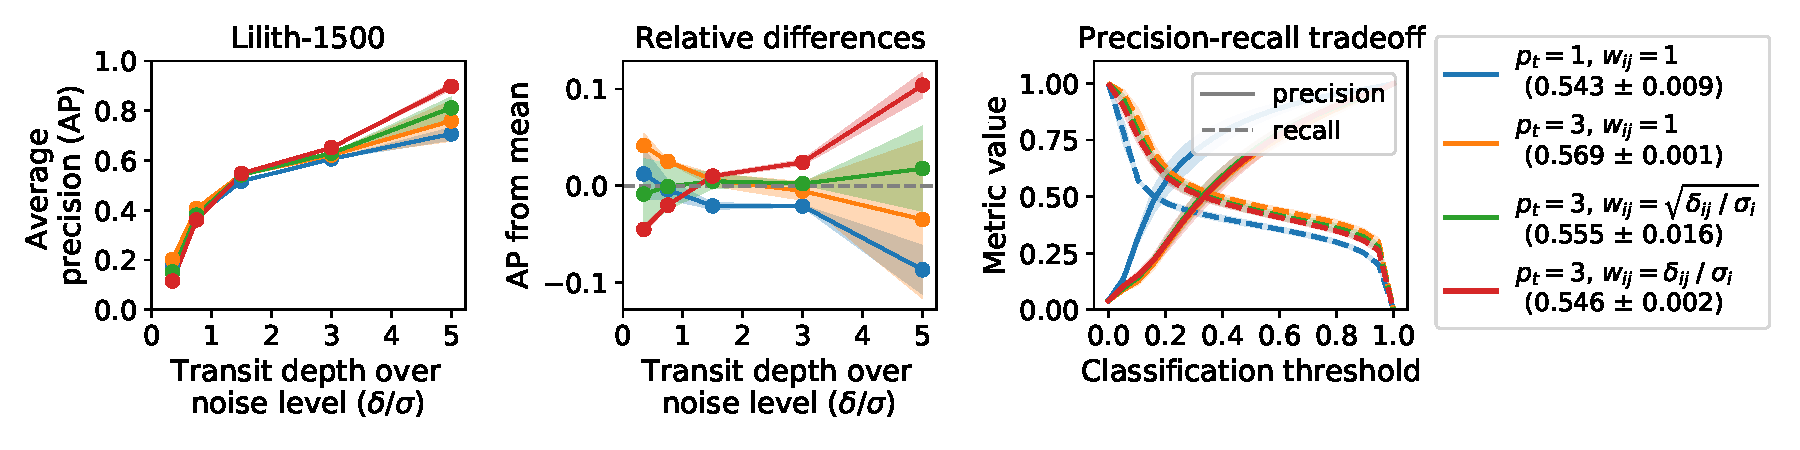
\includegraphics[width=0.97\linewidth]{Experiments/Figures/Models/lilith1500_AP_weighting.pdf}
    \caption{The effect of different weighting schemes on the AP evaluated on the test split of Lilith-1500. The results are similar to those obtained using LCSim-1500 in the sense that a positive weight $p_t$ larger than 1 seems beneficial for the AP, and that $w_{ij}$ can be used to shift the focus of the neural network towards specific transit samples.}
    \label{fig:lilith_weighting}
\end{figure}
